\documentclass{article}
\usepackage[a4paper]{geometry}
\usepackage{graphicx}
\usepackage[utf8]{inputenc}
\usepackage{subcaption}
\usepackage{placeins}
\usepackage{wrapfig}
\usepackage{float}
\usepackage{hyperref}
\usepackage{minted}

\graphicspath{{./images/}}

\title{Aplicație pentru managementul unei biblioteci}
\author{
    Mițca Dumitru\\
    Grupa 1311A\\
    Coordonator: Mironeanu Cătălin\\
    \emph{Facultatea de Automatică și Calculatoare}
}
\date{2023}

\begin{document}
    \maketitle
    \hypersetup{linkbordercolor=1 1 1}
    \renewcommand*\contentsname{Cuprins}
    \tableofcontents
    \hypersetup{linkbordercolor=1 0 0}

    \newpage

    \section{Descrierea proiectului}

    \subsection{Scopul aplicației}

    Aplicația a fost concepută pentru management-ul unei biblioteci, cu funcționalități utile și pentru
    oamenii care doar împrumută cărți, cât și pentru bibliotecari.

    Astfel, pentru utilizatorii normali, sunt oferite următoarele funcționalități:
    \begin{itemize}
        \item abilitatea de a vedea toate cărțile din bibliotecă cu detalii despre carte și autor
        \item abilitatea de a împrumuta o carte, și de a vedea ușor data la care cartea trebuie înapoiată bibliotecii
        \item abilitatea de a-și menține progresul citirii cărții in aplicație prin numărul de capitole citite
    \end{itemize}
    Ca o posibilitate de extindere în viitor a aplicației ar fi adăugare de funcționalități sociale, care ar permite
    utilizatorilor să vadă ce cărți citesc prietenii lor, sau ca o carte să treacă direct de la un utilizator
    la altul.

    Pentru bibliotecari, următoarele funcționalități sunt oferite:
    \begin{itemize}
        \item
    \end{itemize}

    \subsection{Arhitectura proiectului}

    Aplicația se încadrează în categoria aplicațiilor CRUD.

    Aplicația este separată în două programe: un server web și o aplicație desktop care comunică
    prin un API REST. Aplicația desktop nu are acces la baza de date, lucru rezervat exclusiv
    serverului.

    \section{Tehnologii folosite}

    Clientul și serverul sunt amândouă scrise în limbajul de programare Rust\footnote{\url{https://www.rust-lang.org/}},
    lucru care permite împărtășirea definițiilor structurilor folosite în API prin plasarea lor într-o librărie.
    Aceste structuri sunt transmise prin rețea serializându-le în JSON.

    \subsection{Pe back-end}

    Back-end-ul constă într-un server care folosește librăria \emph{axum} pentru expunerea unui API REST,
    librăria \emph{SQLx} pentru comunicația cu baza de date și \emph{SQLite} pentru baza de date în sine.

    \subsubsection*{\emph{axum}\footnote{\url{https://github.com/tokio-rs/axum}}}

    \emph{axum} este un framework pentru servere web ce permite descrierea rutelor expuse de server într-un mod
    declarativ. Acest framework este foarte simplu de utilizat și nu impune mult boilerplate, un exemplu de definire
    a rutelor este:
    \begin{minted}[linenos, breaklines]{rust}
let app = Router::new()
    .route("/", get(root))
    .route("/books", get(books::books))
    .route("/borrow", post(books::borrow))
    .route("/borrowed-by/:user_id", post(books::borrowed_by))
    .nest("/auth", auth::router(pool.clone()))
    .fallback(fallback) // această funcție permite returnarea unui răspuns HTTP cu codul 404 automat pentru rute necunoscute
    .with_state(pool);
    \end{minted}

    \emph{axum} permite și definirea în prototipul funcțiilor formatul în care sunt serializate request-urile de la client
    și răspunsul de la server, ocupându-se automat de serializarea și deserializarea acestora, spre exemplu:
    \begin{minted}[linenos, breaklines]{rust}
async fn create_account(
    State(pool): State<SqlitePool>,
    Json(data): Json<CreateAccount>,
) -> Result<Json<LoginReply>, RouteError>;
    \end{minted}

    \subsubsection*{\emph{SQLx}\footnote{\url{https://github.com/launchbadge/sqlx}}}

    \emph{SQLx} este o librărie care permite conectarea la baze de date și scrierea de interogări SQL.
    Particularitatea acestei librăriei este integrarea cu funcționalitățile pentru asincronicitate în
    Rust\footnote{Totuși, datorită utilizării \emph{SQLite}, back-end-ul nu beneficiază total de acest lucru,
    dar dacă ar fi să schimb baza de date, ar reprezenta un avantaj.} și posibilitatea verificării în timpul
    compilării că interogările scrise de programator sunt în coconcordanță cu schema bazei de date definită
    în fișiere SQL de programator.

    \subsubsection*{\emph{SQLite}\footnote{\url{https://www.sqlite.org/index.html}}}

    \emph{SQLite} este o bază de date relațională, implementată ca o librărie care rulează în același proces ca
    aplicație ce dorește să o folosească. Deși are "lite" în nume, \emph{SQLite} este o implementare completă a
    SQL\footnote{Cu mențiunea că suportul pentru foreign key-uri trebuie activat per conexiune, lucru realizat de
    back-end.} și oferă tranzacției care respectă proprietățile ACID.

    Conexiunea către baza de date este realizată prin intermediul \emph{SQLx}, care pur și simplu apelează funcția
    din \emph{SQLite} pentru deschiderea unei baze de date.

    \subsection{Pe front-end}

    Front-end-ul constă într-o aplicație desktop care folosește \emph{GTK}\footnote{\url{https://www.gtk.org/}}
    și \emph{Adwaita}\footnote{\url{https://gnome.pages.gitlab.gnome.org/libadwaita/doc/}} pentru interfață și
    \emph{Soup}\footnote{\url{https://libsoup.org/libsoup-3.0/index.html}} pentru a realiza request-urile HTTP
    pentru comunicarea cu serverul.

    Am ales să folosesc GTK deoarece există suport foarte bun pentru utilizarea librăriei în Rust și pentru
    că împreuna cu \emph{Blueprints}\footnote{\url{https://jwestman.pages.gitlab.gnome.org/blueprint-compiler/}},
    am putut scrie definiția interfeței grafice într-un mod declarativ, Rust fiind delegat doar pentru logica
    aplicației.

    \emph{Soup} a fost ales deoarece oferă o integrare bună cu GTK, fiind o librărie care își are originile
    în ecosistemul GTK.

    \section{Structura bazei de date}

    \begin{figure}[H]
        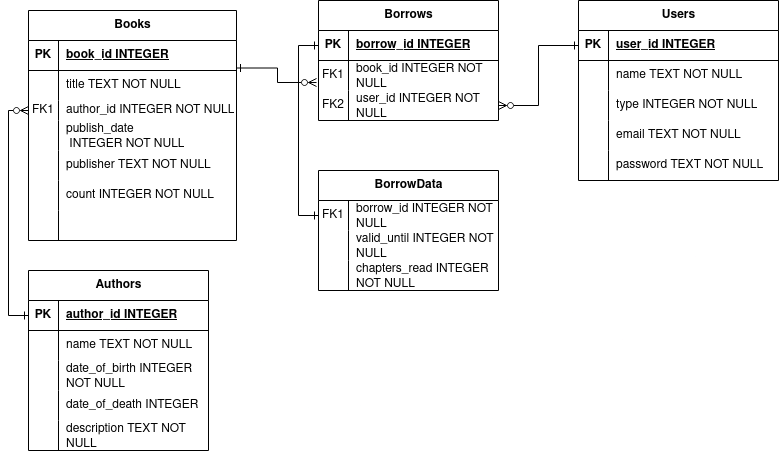
\includegraphics[width=\linewidth]{ER-Diagram}
        \centering
    \end{figure}

    Mențiuni despre normalizarea datelor:
    \begin{itemize}
        \item
    \end{itemize}
    Constrângeri utilizate în baza de date:
    \begin{itemize}
        \item constrângeri de tip cheie primară --- majoritatea tabelelor au chei primare, generate la inserare prin
        funcționalitatea \texttt{AUTOINCREMENT} a \emph{SQLite} și unicitatea lor este asigurată prin utilizarea
        constrăngerii \texttt{PRIMARY KEY} aplicată coloanelor relevante la crearea tabelelor
        \item constrângeri de tip cheie străină --- datorită existența relațiilor între tabele, de exemplu: utilizator
        la cărți împrumutate sau carte la autor; am folosit constrângerea \texttt{FOREIGN KEY} pentru a asigura coerența
        datelor, un exemplu de situație prevenită astfel este ștergerea unui autor când încă există cărți scrise de el
        în baza de date
        \item constrăngeri de tipul \texttt{NOT NULL} --- am folosit astfel de constrângeri pentru că pentru majoritatea
        coloanelor din baza de date, absența valorilor nu are sens
        \item o constrângere de tipul \texttt{UNIQUE} --- în tabela \texttt{BorrowData}, pentru a asigura că nu există mai
        multe înregistrări cu date auxiliare pentru același împrumut
    \end{itemize}

\end{document}
